The strategy is now as follows. The details are left as an exercise.
\begin{enumerate}
	\item The only connected positive definitive Coxeter graphs with $3$
		vertices are paths of length $2$, either with two single edges or
		a single edge and a double edge. The other cases fail to satisfy the
		inequality in the previous lemma.

	\item If there is a triple edge, there cannot be any other multiple edges.

	\item Removing some of the vertices and all of the edges attached to them from
		a positive definite Coxeter graph yields a positive definite Coxeter
		graph.

	\item Contracting an edge of a positive definite Coxeter graph yields a
		positive definite Coxeter graph.

		Similarly, if a positive definite Coxeter graph contains the configuration
		
\begin{tikzpicture}[scale=0.2, dot/.style={circle, fill, inner sep=0pt, outer sep=0pt, minimum size=3pt}]
			\node[dot] (a) at (0, 0) {};
			\node[dot] (b) at (1, 0.5) {};
			\node[dot] (c) at (1, -0.5) {};
			\draw (a) -- (b);
			\draw (a) -- (c);
			\draw[densely dotted] (-1, 0) -- (a);
		\end{tikzpicture}, then collapsing the two edges to
		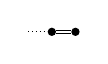
\begin{tikzpicture}[scale=0.3, dot/.style={circle, fill, inner sep=0pt, outer sep=0pt, minimum size=3pt}]
			\node[dot] (a) at (0, 0) {};
			\node[dot] (c) at (1, 0) {};
			\draw[double] (a) -- (c);
			\draw[densely dotted] (-1, 0) -- (a);
		\end{tikzpicture}
		yields a positive definite Coxeter graph.
	\item There are certain invalid graphs:
		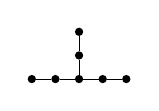
\begin{tikzpicture}[scale=0.3, dot/.style={circle, fill, inner sep=0pt, outer sep=0pt, minimum size=3pt}]
			\node[dot] (a) at (0, 0) {};
			\node[dot] (b) at (0, 1) {};
			\node[dot] (c) at (0, 2) {};
			\node[dot] (d) at (-2, 0) {};
			\node[dot] (e) at (-1, 0) {};
			\node[dot] (f) at (1, 0) {};
			\node[dot] (g) at (2, 0) {};
			\draw (a) -- (b) -- (c);
			\draw (d) -- (e) -- (a) -- (f) -- (g);
		\end{tikzpicture},
		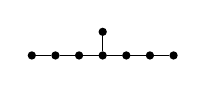
\begin{tikzpicture}[scale=0.3, dot/.style={circle, fill, inner sep=0pt, outer sep=0pt, minimum size=3pt}]
			\node[dot] (a) at (0, 0) {};
			\node[dot] (b) at (0, 1) {};
			\node[dot] (c) at (-3, 0) {};
			\node[dot] (d) at (-2, 0) {};
			\node[dot] (e) at (-1, 0) {};
			\node[dot] (f) at (1, 0) {};
			\node[dot] (g) at (2, 0) {};
			\node[dot] (h) at (3, 0) {};
			\draw (a) -- (b);
			\draw (c) -- (d) -- (e) -- (a) -- (f) -- (g) -- (h);
		\end{tikzpicture},
		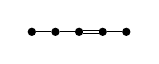
\begin{tikzpicture}[scale=0.3, dot/.style={circle, fill, inner sep=0pt, outer sep=0pt, minimum size=3pt}]
			\node[dot] (a) at (0, 0) {};
			\node[dot] (b) at (1, 0) {};
			\node[dot] (c) at (2, 0) {};
			\node[dot] (d) at (3, 0) {};
			\node[dot] (e) at (4, 0) {};
			\draw (a) -- (b) -- (c);
			\draw[double] (c) -- (d);
			\draw (d) -- (e);
		\end{tikzpicture}, and
		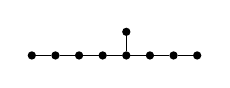
\begin{tikzpicture}[scale=0.3, dot/.style={circle, fill, inner sep=0pt, outer sep=0pt, minimum size=3pt}]
			\node[dot] (a) at (0, 0) {};
			\node[dot] (b) at (1, 1) {};
			\node[dot] (c) at (-3, 0) {};
			\node[dot] (d) at (-2, 0) {};
			\node[dot] (e) at (-1, 0) {};
			\node[dot] (f) at (1, 0) {};
			\node[dot] (g) at (2, 0) {};
			\node[dot] (h) at (3, 0) {};
			\node[dot] (i) at (4, 0) {};
			\draw (f) -- (b);
			\draw (c) -- (d) -- (e) -- (a) -- (f) -- (g) -- (h) -- (i);
		\end{tikzpicture}.
	\item Show that every positive definite Coxeter graph is one of $A_r$, $B_r$,
		$D_r$, $E_6$, $E_7$, $E_8$, $F_4$, $G_2$.
\end{enumerate}
